\documentclass[12pt, letterpaper]{article}
\usepackage[utf8]{inputenc}
\usepackage{graphicx}
\graphicspath{ {images/} }

\title{First document}
\author{Michael Fedell \thanks{sourced from overleaf.com}}
\date{January 2019}

\begin{document}
\maketitle
We now have a title prepared with author and date.
This \LaTeX{} document is starting to look great!

Some of the \textbf{greatest}
discoveries in \underline{science}
were made by \textbf{\textit{accident}}.


In case you didn't catch that,

Some of the greatest \emph{discoveries}
in science
were made by accident.

\textit{Some of the greatest \emph{discoveries}
in science
were made by accident.}

\textbf{Some of the greatest \emph{discoveries}
in science
were made by accident.}


The universe is immeense and it seems to be homogeneous, in a large scale, everywhere we look.

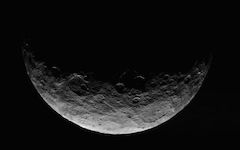
\includegraphics{moon}

There's a picture of the moon above
\end{document}
